
%% bare_jrnl_compsoc.tex
%% V1.4b
%% 2015/08/26
%% by Michael Shell
%% See:
%% http://www.michaelshell.org/
%% for current contact information.
%%
%% This is a skeleton file demonstrating the use of IEEEtran.cls
%% (requires IEEEtran.cls version 1.8b or later) with an IEEE
%% Computer Society journal paper.
%%
%% Support sites:
%% http://www.michaelshell.org/tex/ieeetran/
%% http://www.ctan.org/pkg/ieeetran
%% and
%% http://www.ieee.org/

%%*************************************************************************
%% Legal Notice:
%% This code is offered as-is without any warranty either expressed or
%% implied; without even the implied warranty of MERCHANTABILITY or
%% FITNESS FOR A PARTICULAR PURPOSE! 
%% User assumes all risk.
%% In no event shall the IEEE or any contributor to this code be liable for
%% any damages or losses, including, but not limited to, incidental,
%% consequential, or any other damages, resulting from the use or misuse
%% of any information contained here.
%%
%% All comments are the opinions of their respective authors and are not
%% necessarily endorsed by the IEEE.
%%
%% This work is distributed under the LaTeX Project Public License (LPPL)
%% ( http://www.latex-project.org/ ) version 1.3, and may be freely used,
%% distributed and modified. A copy of the LPPL, version 1.3, is included
%% in the base LaTeX documentation of all distributions of LaTeX released
%% 2003/12/01 or later.
%% Retain all contribution notices and credits.
%% ** Modified files should be clearly indicated as such, including  **
%% ** renaming them and changing author support contact information. **
%%*************************************************************************


% *** Authors should verify (and, if needed, correct) their LaTeX system  ***
% *** with the testflow diagnostic prior to trusting their LaTeX platform ***
% *** with production work. The IEEE's font choices and paper sizes can   ***
% *** trigger bugs that do not appear when using other class files.       ***                          ***
% The testflow support page is at:
% http://www.michaelshell.org/tex/testflow/


\documentclass[10pt,journal,compsoc]{IEEEtran}
%
% If IEEEtran.cls has not been installed into the LaTeX system files,
% manually specify the path to it like:
% \documentclass[10pt,journal,compsoc]{../sty/IEEEtran}





% Some very useful LaTeX packages include:
% (uncomment the ones you want to load)


% *** MISC UTILITY PACKAGES ***
%
%\usepackage{ifpdf}
% Heiko Oberdiek's ifpdf.sty is very useful if you need conditional
% compilation based on whether the output is pdf or dvi.
% usage:
% \ifpdf
%   % pdf code
% \else
%   % dvi code
% \fi
% The latest version of ifpdf.sty can be obtained from:
% http://www.ctan.org/pkg/ifpdf
% Also, note that IEEEtran.cls V1.7 and later provides a builtin
% \ifCLASSINFOpdf conditional that works the same way.
% When switching from latex to pdflatex and vice-versa, the compiler may
% have to be run twice to clear warning/error messages.






% *** CITATION PACKAGES ***
%
\usepackage{amsmath}
\usepackage{amssymb}
\ifCLASSOPTIONcompsoc
  % IEEE Computer Society needs nocompress option
  % requires cite.sty v4.0 or later (November 2003)
  \usepackage[nocompress]{cite}
\else
  % normal IEEE
  \usepackage{cite}
\fi





% *** GRAPHICS RELATED PACKAGES ***
\usepackage{graphicx}
%
\ifCLASSINFOpdf
  % \usepackage[pdftex]{graphicx}
  % declare the path(s) where your graphic files are
  % \graphicspath{{../pdf/}{../jpeg/}}
  % and their extensions so you won't have to specify these with
  % every instance of \includegraphics
  % \DeclareGraphicsExtensions{.pdf,.jpeg,.png}
\else
  % or other class option (dvipsone, dvipdf, if not using dvips). graphicx
  % will default to the driver specified in the system graphics.cfg if no
  % driver is specified.
  % \usepackage[dvips]{graphicx}
  % declare the path(s) where your graphic files are
  % \graphicspath{{../eps/}}
  % and their extensions so you won't have to specify these with
  % every instance of \includegraphics
  % \DeclareGraphicsExtensions{.eps}
\fi
% graphicx was written by David Carlisle and Sebastian Rahtz. It is
% required if you want graphics, photos, etc. graphicx.sty is already
% installed on most LaTeX systems. The latest version and documentation
% can be obtained at: 
% http://www.ctan.org/pkg/graphicx
% Another good source of documentation is "Using Imported Graphics in
% LaTeX2e" by Keith Reckdahl which can be found at:
% http://www.ctan.org/pkg/epslatex
%
% latex, and pdflatex in dvi mode, support graphics in encapsulated
% postscript (.eps) format. pdflatex in pdf mode supports graphics
% in .pdf, .jpeg, .png and .mps (metapost) formats. Users should ensure
% that all non-photo figures use a vector format (.eps, .pdf, .mps) and
% not a bitmapped formats (.jpeg, .png). The IEEE frowns on bitmapped formats
% which can result in "jaggedy"/blurry rendering of lines and letters as
% well as large increases in file sizes.
%
% You can find documentation about the pdfTeX application at:
% http://www.tug.org/applications/pdftex




\hyphenation{op-tical net-works semi-conduc-tor}


\begin{document}
%
% paper title
% Titles are generally capitalized except for words such as a, an, and, as,
% at, but, by, for, in, nor, of, on, or, the, to and up, which are usually
% not capitalized unless they are the first or last word of the title.
% Linebreaks \\ can be used within to get better formatting as desired.
% Do not put math or special symbols in the title.
\title{An Efficient MapReduce Cube Algorithm for Varied Data Distributions}

\author{ \textbf{ Written by Tova Milo and Eyal Altshuler.  \\
Proposed by Maabout Sofian.} \\

Summed up by Lassouani Sofiane and Ouadi Steward.}% <-this % stops a space}

\IEEEtitleabstractindextext{%
% Note that keywords are not normally used for peerreview papers.
\begin{IEEEkeywords}
MapReduce, Data cube,SP-Sketch,Skewed  \ldots
\end{IEEEkeywords}}


% make the title area
\maketitle


\IEEEdisplaynontitleabstractindextext
\IEEEpeerreviewmaketitle



\section{Introduction}\label{sec:introduction}

A data cube is a higher-dimensional structure which allows finding insights in data analysis. An example of a data cube is given in Appendix A. A more detailed definition will be given in the following section. Each dimension represents an attribute in the database table. Data cube is a powerful data analysis tool allowing an easy look at the data (allows to look at complex data in a simple format). Data cube is very expensive to compute in particular when the input relation is large eg: imagine a table with n fields, we'll have ${2^n}$ tables in the calculation of the data cube. Very useful in data analysis, research has been conducted in this context in order to find less expensive calculation solutions. In this article a data cube calculation algorithm is presented as the most efficient using MapReduce, the popular paradigm for large-scale data processing.


Existing techniques suffer from the way they determine skewed data, and their performance depends on how exactly the data is skewed. This algorithm uses sampling to identify skews, and a dedicated data structure called the Skews and Partitions Sketch (SP-Sketch for short). The SP-Sketch is compact in size, fast to compute, records all needed information for identifying skews and distributes tasks between machines optimally.

\section{Context}\label{sec:context}

This article deals with efficient data cube computation in a MapReduce environment. Compute the data cube efficiently allows faster analysis of the data, as we do not have anymore to compute over ${2^n}$ data but only on the data that are in the data cube. So, data cube reduces response time by analyzing only a small part (the one we are interested in) of the data. 

A MapReduce algorithm may have one or more phases. Those phases are divided into two parts or functions : map function and reduce function. A map function applies one function to each data entry and then passes intermediate data to the reduce function. The reduce function operates on those input data, reduces the number of given data and then outputs those data. An efficient MapReduce program should have a small amount of data passing through the network.

Before going further, let us give the definition of a relation \textbf{R}, tuple, projection, dimension attribute and measure attribute with an example.
In the example below, we suppose that the measure value and the attributes values can fit in a machine's main memory.  

\textit{EXEMPLE 1. We consider a relation \textbf{R} describing the number of people having the same name in different departments of FRANCE over the years. \textbf{R} has three dimension attributes: A1 = name , A2 = department , A3 = year, and a measure attribute B  = number\_of\_people. For example, in \textbf{R}, we can have this tuple t=(David,Gironde,2015,500) which describes the fact that in 2015, there were 500 people with the name David in Gironde. The projection of t onto the dimensions name  and year is denoted (David, *, 2015).}

Now we have defined the different steps of a MapReduce algorithm and given a definition of a relation, let us define a data cube (an example of a data cube is provided in Appendix A). The data cube of a relation \textbf{R} is a set of relations, each of which can be grouped-by on an attribute. 

In order to define a cuboid and \textbf{cube group} (\textbf{c-group} for short), we will also use an example. We have to keep in mind that we have \textbf{tuples} of a relation \textbf{R} that are in \textbf{c-groups}, and those \textbf{c-groups} are in a specific \textbf{cuboid}

\textit{EXEMPLE 2. Let us take back our previous example, the data cube of \textbf{R} consists of 8 \textbf{cuboids}, including for instance the \textbf{cuboids} \textbf{C1} = (name, department,* ) and \textbf{C2} = (*, *, *). The \textbf{cuboid} \textbf{C1} is obtained by grouping the tuples in \textbf{R} by name
 and department, applying an aggregation function (sum,count,max) to the measure attribute of each group. Two \textbf{c-groups} in \textbf{C1} may be \textit{c1} = (David, Gironde, *) and \textit{$c1 \prime$} = (David,Guyane,*). \textit{c1} (resp. \textit{$c1 \prime$}) is generated by aggregating the set of tuples set(\textit{c1}) (resp.set(\textit{$c1 \prime$})) of \textbf{R} that includes all tuples describing the number of people having the name David in Gironde and Guyane. The \textbf{cuboid} \textbf{C2} consists of a single value \textit{c2} obtained by aggregating the measure attribute of all the tuples
in \textbf{R}. Here set(c2) consists of all the tuples in \textbf{R}. Note
that the tuple t = (David,Guyane, 2014, 120) contributes to both c1 and c2.}

We want to compute data cube efficiently. If many tuples have the same value, for instance (*,Gironde,2015) when projected on the department and year attributes and these tuples cannot fit in a machine's main memory, then the cuboid of these tuples is defined as skewed by the authors.

\section{Contribution}\label{sec:contribution}

The authors have contributed in five different ways improving the data cube algorithm.

First the authors have provided a model which defines the notion of skewed c-groups. The authors highlight that in order to create an efficient MapReduce algorithm, they should take into account that notion and exploit it. The authors define a group as each tuple that matches a "group-by" function and a skewed group as data that are too big to fit in a machine's main memory (RAM).

Secondly, the authors have proposed a novel data structure : SP-Sketch (Skews and Partitions Sketch). This structure is the crux of their algorithm, it is small enough to fit in a machine's main memory and is fast to compute. Moreover, it grabs all needed information faster to decide whether or not a particular group is skewed in order to make an efficient partitioning. 

Besides, the authors have proposed SP-Cube Algorithm. This algorithm, which is their \textbf{main} contribution, uses their data structure SP-Sketch and allows them to efficiently partially compute a group in the map phase if that group is skewed or to send non skewed groups to reducers. Those reducers will then compute all non skewed groups and aggregate the groups that have been partially computed by the mappers.

Moreover, the authors have proposed a theoretical analysis which demonstrates the efficiency of their algorithm in terms of machine's main memory size and data transferred size. The authors show that the size of data transferred between the mappers and the reducers can be exponential with respect to the number of dimensions. But in common cases, the size of the data is only polynomial with respect to the number of dimensions.

Finally, the authors have done different experiments to compare their solution to previous ones. They have done their experiments with two real-life data sets as well as synthetic data. The authors then focus on particular phases of the algorithm namely, map phase and reduce phase and also have a look at the whole computing process. And they have found that their solution outperforms previous ones, achieving between 20\% - 300\% better running time and smaller network traffic. 

%\subsection{Subsection Heading Here}
%Subsection text here.

\section{Discussion}\label{sec:discussion}
In order to understand the computational complexity of the cube in MapReduce we will present a naive algorithm and describe its disadvantages

\subsection{MapReduce Cubing-Naive approach }

Let's take an example of naive calculation algorithm of the cube, assume a relation \textbf{R} with dimension attributes and a measure attribute R($\textrm{A}_\textrm{1}$,$\textrm{A}_\textrm{2}$ ... $\textrm{A}_\textrm{n}$, M), written on a distributed file on which the tuples of data will be read, To construct the cube, one must assume all the possible combinations of this relation R. The algorithm begins with a map phase where each tuple t is projected onto each subset of its dimensions. A pair (key, value) is issued, where the key is the projected tuple and the value is the measurement attribute of t, the outputs of the mapper are then sent to a reducer which is responsible for reducing all tuples with the same key. Note that all tuples with the same key are sent to the same reducer that is chosen by the MapReduce framework using a hash function h to share the keys on the different existing reducers.

The first problem encountered with this naive method is that we must do as much mapping and as many reducers as there are possible combinations of the relation R, to construct the table $\textrm{R}_\textrm{n}$($\textrm{A}_\textrm{i}$, M), $\textrm{R}_\textrm{m}$($\textrm{A}_\textrm{i}$$\textrm{A}_\textrm{j}$ M), i$\ne$J, ...

The second problem encountered with the naive algorithm is its sensitivity to sets carrying the same key, especially when this set is voluminous. Assume a relation R($\textrm{A}_\textrm{1}$,$\textrm{A}_\textrm{2}$ ... $\textrm{A}_\textrm{n}$, M), now suppose that many tuples that have the value (*, $\textrm{A}_\textrm{2}$, M) when projected on attributes $\textrm{A}_\textrm{2}$ and M, ensure that the reducer that will handle this group will not have to handle many other groups because some keys may be more present than others. To better balance the reducers load, we would have to divide the keys according to their frequency in order to distribute the load between the reducers, which leads us to deduce that the real problem is to find a hash function that does the distribution of keys taking into account their frequency. This is what the authors have sought to solve in order to prevent saturation of the capacity of the reducers which will not be able to perform aggregation in the main memory, and performance will suffer

Consider \textbf{m} the partial input size of the machines, we know that a group \textbf{g} is skewed if the cardinality of its set is greater than \textbf{m}, and since the aggregation cannot fit in the reducer's main memory, the phase of Reduce involves I/O between main memory and disk, which makes the overall calculation slower. In order to remedy, this algorithm detects all skewed groups and partially aggregates them already at the map phase, before sending them to the reducer. Thus, this algorithm allows reducing computation time.

The major issue of the calculation in MapReduce is the large traffic flowing over the network. It is described in the article that much of this communication is redundant and can be avoided. That would help decrease the network traffic.

Like \cite{32} and \cite{26}, the authors use sampling in their algorithm, \cite{32} use it to design efficient sorting in MapReduce, while  \cite{26} use it to determine if a given cuboid contains biases. In the article, sampling is used for partitioning purposes, identifying group bias and not only detect their existence, so it builds the SP-Sketch structure that successfully captures all skewed groups.

\subsection{THE SP-CUBE ALGORITHM }

Before starting to explain the algorithm, it is to be noted that the main disadvantage of MapReduce is how the workload between all the reducers is balanced, because some of the aggregated groups as well as the computed cube itself may be very large, and thus balancing computation and avoiding the generation of large intermediate data is not trivial.This is what the authors seek to achieve in this algorithm. 


The algorithm described in the article is called SP-CUBE. It consists of two phases, the first consists in constructing the data structure the SP-Sketch and the second phase focuses on the calculation of the cube based on the former.
Let us remind that the SP-Sketch contains all the necessary information on the data in order to decide whether a given group is biased or not, by saving the elements of the biased group in a hash table. The key of each element in the hash table is the (concatenated) value of the dimension attributes of the biased group. So to decide whether a group is biased or not, the algorithm checks whether the group key (concatenated value, its attributes) can be found in the table. If the group key is found, the mapper will compute the data before sending it to the reducer. If the group key is not found, the group is considered as not biased and thus send directly and efficiently to a chosen reducer without computing it.

\section{Related Work}\label{sec:related}
Other people have also worked on algorithms to improve the efficiency of computing on data cubes. 

For example, the following articles : \cite{ksbeyer,myelta,kaross,ssarawagi,yzhao} speak about developing efficient algorithms for cube computation.

\cite{aabello,slee,anandi,svemuri} also talk about developing efficient algorithms for cube computation but also about algorithms that are implemented in a MapReduce environment. Some of those algorithms have even been implemented in Pig \cite{pig} and Hive \cite{hive}. Pig  is a high-level platform for creating programs that run on Apache Hadoop \cite{hadoop}. Hive  is a data warehouse infrastructure built on top of Hadoop for providing data summarization, query, and analysis. Hive gives an SQL-like interface to query data stored in various databases and file systems that integrate with Hadoop.

So, all those algorithms provide valuable assets. In \cite{anandi} the algorithm's performance
is demonstrated and shown to outperform previous cube algorithms implemented on top of MapReduce but all of those algorithms still suffer from sensitivity to the distribution of the input data and their performance depends heavily on whether or not, and how exactly, the data is skewed.
\section{Conclusion}\label{sec:conclusion}
In this article a data cube algorithm for large sets of data is presented as the most efficient compared to the already existing solutions.
This algorithm uses a data structure called SP-Sketch, which records all the information needed to detect biases and effectively distributes the workload between machines. This algorithm also has the particularity of reducing the network flow which can be generated by the communication between machines.



\appendices
\section{Example of one Data cube}
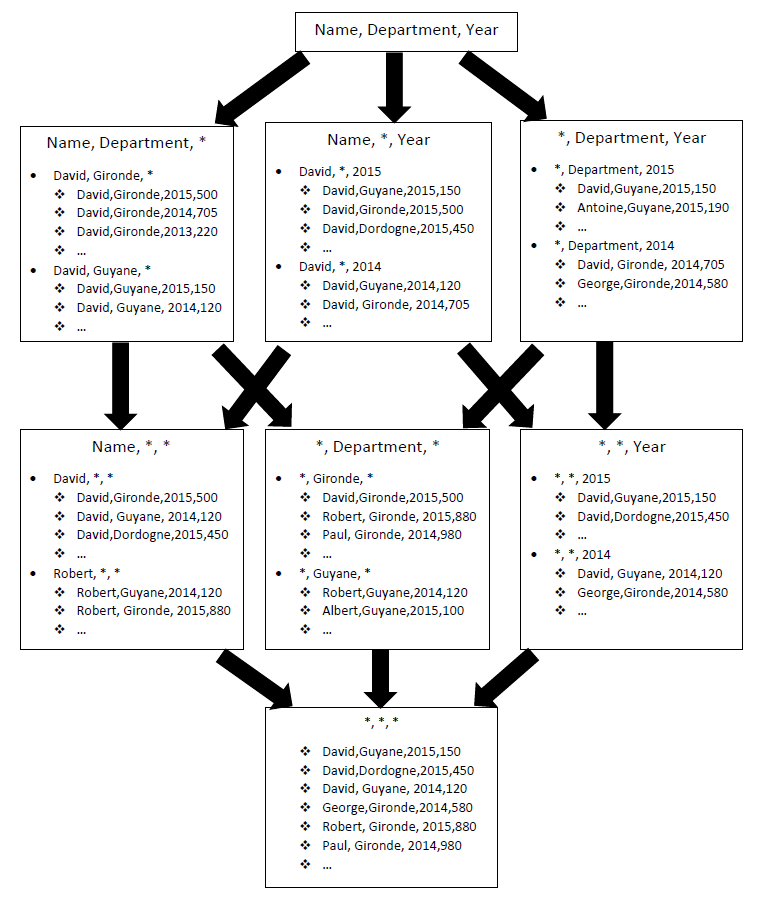
\includegraphics[scale=0.5]{data_cube_example}
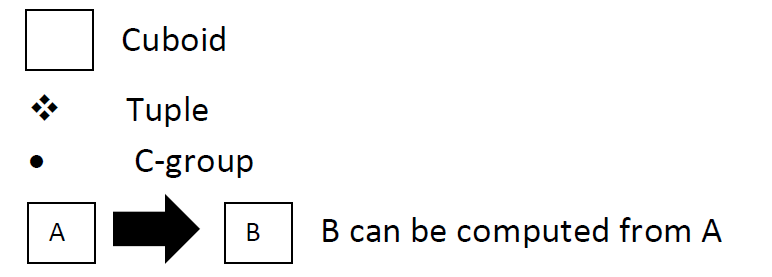
\includegraphics[scale=0.25]{legend_data_cube}


\begin{thebibliography}{3}

 \bibitem{ksbeyer} 
  K. S. Beyer and R. Ramakrishnan. Bottom-up
computation of sparse and iceberg cubes. In SIGMOD,
pages 359-370, 1999.

\bibitem{myelta}
M. Fang, N. Shivakumar, H. Garcia-Molina,
R. Motwani, and J. D. Ullman. Computing iceberg
queries efficiently. In VLDB, pages 299-310, 1998.

\bibitem{kaross}
K. A. Ross and D. Srivastava. Fast computation of
sparse datacubes. In VLDB, pages 116-125, 1997.

\bibitem{ssarawagi}
S. Sarawagi, R. Agrawal, and N. Megiddo.
Discovery-driven exploration of OLAP data cubes. In
EDBT, pages 168-182, 1998.

\bibitem{yzhao}
Y. Zhao, P. Deshpande, and J. F. Naughton. An
array-based algorithm for simultaneous
multidimensional aggregates. In SIGMOD, pages
159-170, 1997.




\bibitem{aabello}
A. Abello, J. Ferrarons, and O. Romero. Building
cubes with mapreduce. In DOLAP, pages 17-24, 2011.

\bibitem{slee}
S. Lee, J. Kim, Y. Moon, and W. Lee. Efficient
distributed parallel top-down computation of ROLAP
data cube using mapreduce. In Data Warehousing and
Knowledge Discovery - 14th International Conference,
DaWaK 2012, Vienna, Austria, September 3-6, 2012.
Proceedings, pages 168-179, 2012.

\bibitem{anandi}
A. Nandi, C. Yu, P. Bohannon, and R. Ramakrishnan.
Data cube materialization and mining over
mapreduce. IEEE Trans. Knowl. Data Eng.,
24(10):1747-1759, 2012.

\bibitem{svemuri}
S. Vemuri, M. Varshney, K. Puttaswamy, and R. Liu.
Execution primitives for scalable joins and
aggregations in map reduce. PVLDB,
7(13):1462-1473, 2014.


\bibitem{hive}
Apache hive.
\\\texttt{ https://www.hive.com}

\bibitem{pig}
Apache pig. 
\\\texttt{ https://pig.apache.org}

\bibitem{hadoop}
Apache Hadoop
\\\texttt{ http://hadoop.apache.org}

\bibitem{32}
Y. Tao, W. Lin, and X. Xiao. Minimal mapreduce algorithms. In SIGMOD, pages 529–540, 2013.
\\\texttt{}

\bibitem{26}
A. Nandi, C. Yu, P. Bohannon, and R. Ramakrishnan. Data cube materialization and mining over mapreduce. IEEE Trans. Knowl. Data Eng., 24(10):1747–1759, 2012. 
\\\texttt{}
\end{thebibliography}
 

\end{document}


